

\documentclass[letterpaper, 11pt]{article}



\usepackage[margin=1in]{geometry}
\usepackage{setspace}\onehalfspace
\usepackage{microtype}


\usepackage{amsmath} \allowdisplaybreaks
\usepackage{amssymb}
\usepackage{amsthm} 
%\theoremstyle{definition}    % if you want normal upright font styles for theorems.
\newtheorem{theorem}{Theorem}
\newtheorem{lemma}{Lemma}
\newtheorem{assumption}{Assumption}
\newtheorem{proposition}{Proposition}
\newtheorem{definition}{Definition}


\usepackage{natbib}
\usepackage{bibentry}


\usepackage{booktabs} % for toprule, midrule, bottomrule
\usepackage{graphicx}
\usepackage{appendix}
\usepackage[counterclockwise]{rotating} % for sidewaystable
\usepackage{subcaption} % for subfigure
\usepackage[normalem]{ulem} % for uline

\usepackage{url}
\usepackage[bookmarks=false,hidelinks]{hyperref}

\usepackage{tikz}
\usetikzlibrary{automata,calc,trees,positioning,arrows,chains,shapes.geometric,%
decorations.pathreplacing,decorations.pathmorphing,shapes,%
matrix,shapes.symbols,plotmarks,decorations.markings,shadows}

\usepackage{pgf}
\pgfdeclarelayer{background}
\pgfdeclarelayer{foreground}
\pgfsetlayers{background,main,foreground}


%\usepackage{authblk}
%\renewcommand\Authfont{\sf\Large}
%\renewcommand\Affilfont{\rm\small}





%%%%%%%%%%%%%% MACRO %%%%%%%%%%%%%%%%%%%%%%%%%%%%%%%%%%%%%%
\newcommand{\email}[1]{{\href{mailto:#1}{\nolinkurl{#1}}}}

\usepackage{bm}
\renewcommand{\vec}[1]{\bm{#1}}
\newcommand{\mat}[1]{\bm{#1}}

\usepackage{xcolor}
\newcommand{\note}[1]{{\Large\bf#1}}
\newcommand{\bluenote}[1]{{\Large\color{blue}#1}}
\newcommand{\rednote}[1]{{\Large\color{red}#1}}

\usepackage{etoolbox}
% To use, for example, \Ac for \mathcal{A}.  Requires "etoolbox" package
\makeatletter
\def\do#1{\@namedef{#1c}{\ensuremath{\mathcal{#1}}}}
\docsvlist{A,B,C,D,E,F,G,H,I,J,K,L,M,N,O,P,Q,R,S,T,U,V,W,X,Y,Z}
\makeatother

\def\Eb{\mathbb{E}}
\def\Rb{\mathbb{R}}
%\def\response{[$\Longrightarrow$]}

\newenvironment{response}
{ [$\Longrightarrow$]\sf }
{ \hfill \rule{1ex}{1ex} }

\newcommand{\dx}{\mathop{}\!\mathrm{d}x}
\newcommand{\dy}{\mathop{}\!\mathrm{d}y}
\newcommand{\dz}{\mathop{}\!\mathrm{d}z}
\newcommand{\dt}{\mathop{}\!\mathrm{d}t}

\renewcommand{\bar}[1]{\mkern 1.5mu\overline{\mkern-1.5mu#1\mkern-1.5mu}\mkern 1.5mu}

%%%%%%%%%%%%%%%%%%%%%%%%%%%%%%%%%%%%%%%%%%%%%%%%%%%%%%%%



\title{A LaTeX Template for Writing Papers}
\author{Author Name \and Another Name \and Changhyun Kwon\footnote{Corresponding Author: \email{chkwon@buffalo.edu}}}
\date{Department of Industrial and Systems Engineering\\University at Buffalo\\[0.5cm] February 16, 2015}

%\usepackage{showlabels} 
%\usepackage[final]{showlabels}


\begin{document}
\maketitle

\begin{abstract}
This document provides some useful tips as well as serve a template for writing a paper in LaTeX. To understand how LaTeX works, you should compare the source code and the output PDF.\\
\noindent\textbf{Keywords:} keyword1; keyword2; keyword3
\end{abstract}



\section{Text} \label{sec:paragraph}
In LaTeX, just enter an empty line for a new paragraph.

Like this. blah blah blah blah blah blah blah blah blah blah blah blah blah blah blah blah blah blah blah blah blah blah blah blah blah blah blah blah blah blah blah blah blah blah blah blah blah blah blah blah blah blah blah blah blah blah blah blah.

\uline{Don't use double backslashed for a new paragraph.} Backslashed will be used in tables and equations only. Some random text here, there, and everywhere. Some random text here, there, and everywhere. Some random text here, there, and everywhere. Some random text here, there, and everywhere. Some random text here, there, and everywhere.  \\
\uline{If you use double backslashes for a new paragraph, it will look very bad.} Some random text here, there, and everywhere. Some random text here, there, and everywhere. Some random text here, there, and everywhere. Some random text here, there, and everywhere. Some random text here, there, and everywhere. 

If you want to \emph{emphasize} some \emph{words}, use \emph{emph}, instead of \textit{textit}.




\section{Citation} \label{sec:citation}

\begin{itemize}
\item Textual citation: \citet{Kwon2013rsp}
\item Parenthetical citation: \citep{Kwon2013rsp}
\item Multiple parenthetical citations: \citep{Bertsimas2004,Chaerani2005,Kouvelis1996,gabrel2012recent}
\item If you need multiple \emph{textual} citations, it is better to write: \citet{Bertsimas2004}, \citet{Chaerani2005}, \citet{Kouvelis1996}, and \citet{gabrel2012recent}, instead of \citet{Bertsimas2004,Chaerani2005,Kouvelis1996,gabrel2012recent}.

\end{itemize}

See them in action:
\begin{quote}
In this paper, we propose a robust optimization framework for the routing methods based on the CVaR risk measure, assuming that data are uncertain within given sets. The proposed robust optimization method is closely related to robust shortest path (RSP) problems, which find a path that minimizes the worst-case travel cost with an uncertain set of travel cost data. When the uncertain set is box-constrained, the RSP problem can be solved in polynomial time \citep{Bertsimas2003network}, while the problem is NP-hard when the uncertain set is an ellipsoid \citep{Bertsimas2004,Chaerani2005} and a set of scenarios \citep{Kouvelis1996}. We refer readers to \citet{ben2009robust} and \citet{gabrel2012recent} and references therein for general robust optimization methods. 
\end{quote}




\section{Math} \label{sec:math}
Inline equations can be like $\sum_{j:(i,j)\in\Ac} x_{ij}$.

A single line equation:
\begin{equation}
	\sum_{j:(i,j)\in\Ac} x_{ij} = 1 \quad \forall i\in\Nc \label{node_constraint1}
\end{equation}
I used $\Ac$ as a shorthand for $\mathcal{A}$. 

Try to give some consistency in your notation. I usually use calligraphic letters to denote sets like set of nodes $\Nc$, set of arcs $\Ac$, set of shipments $\Sc$ as in $n\in\Nc$ or $\sum_{s\in\Sc} z_s$, and so on. Lower-case alphabets for variables like $x_{ij}$, $y_i$, and $z_j$. Upper-case roman alphabets like $N$, $A$, and $S$ for constants as in $n=1,...,N$ or $\sum_{s=1}^S x_s$. 

I usually use lower-case Greek letters for dual variables: $\lambda_i$, $\rho_j$, etc. Upper-case Greek letters may be some special sets or sets of dual variables: $\Lambda$, $\Theta$, etc.

Multiple lines:
\begin{align}
	\sum_{j:(i,j)\in\Ac} x_{ij} = 1 \quad & \forall i\in\Nc \label{node_constraint2} \\
	\sum_{j:(i,j)\in\Ac} y_{ij} = 1 \quad & \forall i\in\Nc \nonumber \\
	\sum_{j:(i,j)\in\Ac} z_{ij} = 1 \quad & \forall i\in\Nc \label{node_constraint3} \\
	\sum_{j:(i,j)\in\Ac} \omega_{ij} = 1 \quad & \forall i\in\Nc \label{node_constraint4} \\
	\sum_{j:(i,j)\in\Ac} \eta_{ij} = 1 \quad & \forall i\in\Nc \label{node_constraint5} 
\end{align}

A single equation that stretches to multiple lines
\begin{multline}
	\sum_{j:(i,j)\in\Ac} x_{ij} + \sum_{j:(i,j)\in\Ac} x_{ij} + \sum_{j:(i,j)\in\Ac} x_{ij} \\
	+ \sum_{j:(i,j)\in\Ac} x_{ij} +	\sum_{j:(i,j)\in\Ac} x_{ij} + \sum_{j:(i,j)\in\Ac} x_{ij} \\
	+ \sum_{j:(i,j)\in\Ac} x_{ij} +	\sum_{j:(i,j)\in\Ac} x_{ij} + \sum_{j:(i,j)\in\Ac} x_{ij} \\
	+ \sum_{j:(i,j)\in\Ac} x_{ij} + \sum_{j:(i,j)\in\Ac} x_{ij} = 1 
\end{multline}

When you want cross-referencing, do this: \eqref{node_constraint1}, or \eqref{node_constraint2}--\eqref{node_constraint5}.

If you don't want numbering, just add *, like:
\begin{equation*}
	\sum_{j:(i,j)\in\Ac} x_{ij} = 1 \quad \forall i\in\Nc
\end{equation*}
or
\[
	\sum_{j:(i,j)\in\Ac} x_{ij} = 1 \quad \forall i\in\Nc
\]
or
\begin{align*}
	\sum_{j:(i,j)\in\Ac} x_{ij} = 1 \quad & \forall i\in\Nc \\
	\sum_{j:(i,j)\in\Ac} y_{ij} = 1 \quad & \forall i\in\Nc \\
\end{align*}

Please do not use words for variables. 
\begin{itemize}
\item Don't:
	\[
		counter_1 = 3 + 10 
	\]
	where $counter_1$ may be confused with $c \times o \times u \times n \times t \times e \times r_1$.

\item Instead do:
	\[
		c_i = 3 + 10
	\]
	or
	\[
		\text{counter}_1 = 3 + 10
	\]
	or
	\[
		\textsf{counter}_1 = 3 + 10
	\]
depending on the context.
\end{itemize}


You can use $\vec{x}$ as a vector of $x_{ij}$. Some matrices $\mat{A}$ and $\mat{B}$.

Some vectors are here:
\[
	\vec{y} = \begin{bmatrix} 3 \\ 2 \\ 1 \end{bmatrix}, \qquad
	\vec{z} = \begin{bmatrix} z_1 \\ z_2 \\ \vdots \\ z_n \end{bmatrix}
\]
A matrix is here:
\[
	\mat{A} = \begin{bmatrix} a_{11} & \cdots & a_{22}  \\
							  \vdots & \ddots & \vdots  \\
							  a_{1n} & \cdots & a_{nn}  \end{bmatrix}
\]
If you like curly brackets:
\[
	\mat{A} = \begin{pmatrix} a_{11} & \cdots & a_{22}  \\
							  \vdots & \ddots & \vdots  \\
							  a_{1n} & \cdots & a_{nn}  \end{pmatrix}
\]



\section{Theorem}

You can write a theorem with a proof.

\begin{theorem} \label{thm:fundamental}
If one is not drunken, the following is true:
\begin{equation}
	1 + 2 = c
\end{equation}
where $c$ is a constant that represents 3.
\end{theorem}
\begin{proof}
Obvious.
\end{proof}

\begin{definition}
Definition...............
\end{definition}

\begin{lemma}
Lemma............
\end{lemma}
\begin{proof}
We can prove this lemma by using Theorem \ref{thm:fundamental}.
\end{proof}



\section{Tables}


\begin{table} \centering
\caption{The table caption is above the table. Text to the left, numbers to the right. }
\label{tbl:example}
\begin{tabular}{l l r r}
\toprule
Name		& Location		&  Number	& Number \\
\midrule
Michael		& Chicago			&      10   &   3.190  \\
Sara		& Montreal			&     110   & 123.148  \\
Sandra		& LA				&    1210   &   3.000  \\
Alexander	& San Francisco		&       8   &   0.000  \\
\bottomrule
\end{tabular}
\end{table}

\begin{table} \centering
\caption{A bad presentation.}
\label{tbl:bad_example}
\begin{tabular}{c c l l}
\toprule
Name		& Location		&  Number	& Number \\
\midrule
Michael		& Chicago			&      10   &   3.190  \\
Sara		& Montreal			&     110   & 123.148  \\
Sandra		& LA				&    1210   &   3.000  \\
Alexander	& San Francisco		&       8   &   0.000  \\
\bottomrule
\end{tabular}
\end{table}

When you prepare tables, please just ignore the positioning of tables in the final PDF file. I put the code for Table \ref{tbl:example} above this text and the code for Table \ref{table:8-node} below this text. Their actual locations in the output PDF file will be determined by LaTeX. Table \ref{tbl:bad_example} is a bad presentation of Table \ref{tbl:example}. Tables \ref{tbl:example}--\ref{table:8-node} are small tables. If you have a big table like Table \ref{table:EDOandLINGO}, then you can use `\texttt{sidewaystable}'. However, it is best to redesign the table and not to use sideway tables. Think one more time to decide if you really need such a big table to make your arguments clear. 


\begin{table}  \centering
\caption{Arc attributes for the 8-node network, with $\rho_a$: the population density along arc $a$ and $c_a(v_a)=A_a(1 + 0.15{(v_a/l_a)}^4)$.} 
\label{table:8-node}%
\begin{tabular}{rrrrr}
\toprule
\multicolumn{2}{c}{\text{Arc $a$}}   & 				&			&			\\
\cmidrule(lr){1-2}
Start & End & $A_a$ & $l_a$ & $\rho_a$ \\
\midrule
    1 &   2 &     6 &   900 &      701\\
    1 &   3 &     4 &  1400 &    11193\\
    2 &   3 &     6 &   700 &     1701\\
\bottomrule
\end{tabular}
\end{table}


\begin{sidewaystable}
\caption{A sideway table.}
\label{table:EDOandLINGO}
\begin{tabular}{r rrrr rrrr rrrr}
\toprule
& \multicolumn{4}{c}{LINGO} & \multicolumn{4}{c}{Modified EDO} & \multicolumn{4}{c}{2-Step EDO} \\
\cmidrule(lr){2-5} \cmidrule(lr){6-9} \cmidrule(lr){10-12} 
Case &     Solution &    Risk &     Toll &   Run   &    Risk &    Toll &   Run & Objective   &    Risk &    Toll &    Run & Objective \\
     &         Type &         &  Revenue &  Time   &         & Revenue &  Time &  Gap (\%)   &         & Revenue &   Time &  Gap (\%) \\
\midrule
   1 &       Global & 2469.86 &        0 & 4 sec   & 2945.94 &  703.28 & 8 sec &     47.75   & 2469.86 &    1.96 & 14 sec &      0.08 \\
\bottomrule
\end{tabular}
\end{sidewaystable}





\section{Figures} \label{sec:figures}


\begin{figure} \centering
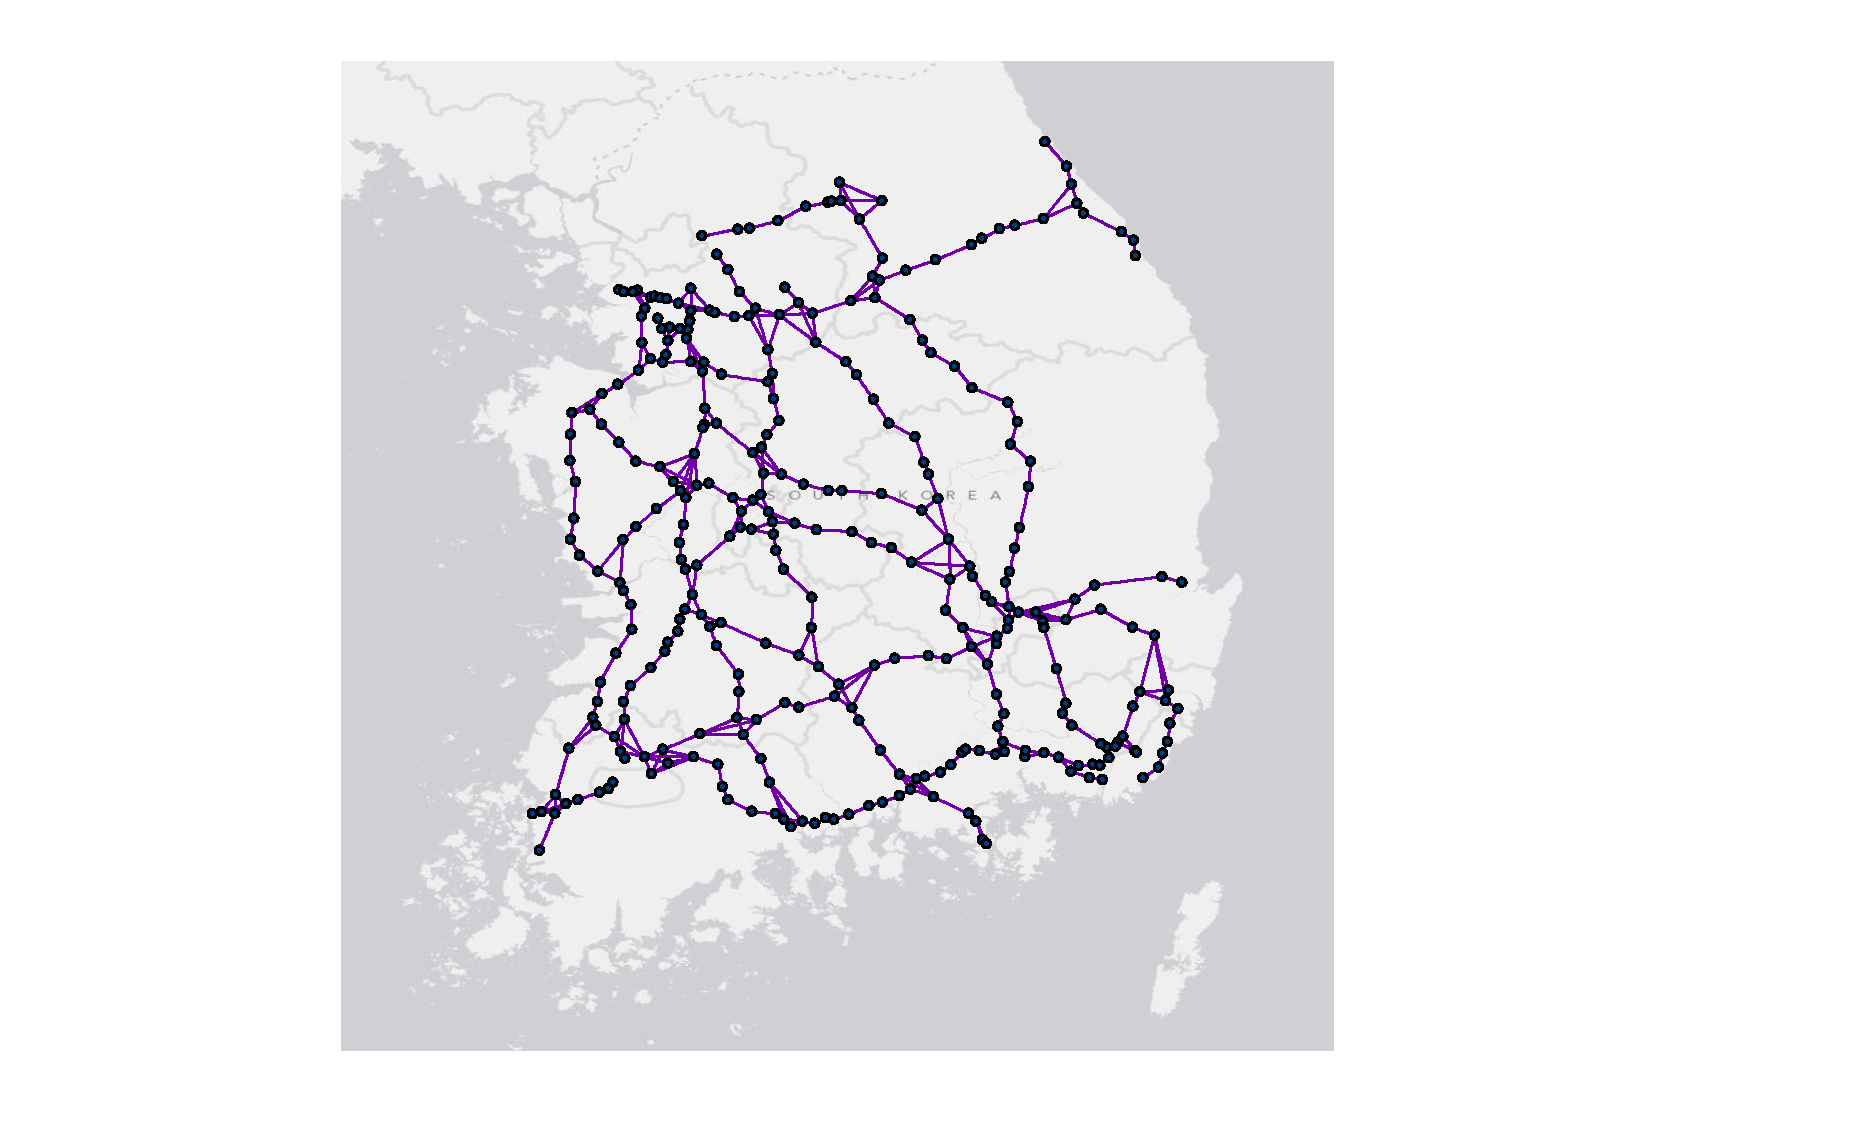
\includegraphics[width=0.45\textwidth]{map}
\caption{Figure caption is below the figure.}
\label{fig:map}
\end{figure}

For figures, it is better to put the caption below the figure. See Figure \ref{fig:map}. Whenever possible, you should save your figure as a vector-based PDF file. PDF files that were converted from a JPG file do not look good. Compare Figures \ref{fig:map-pdf} and \ref{fig:map-jpg}. As you have already seen in Figure \ref{fig:side-by-side}, you can put figures side by side.

If you are using \texttt{MATLAB} to generate figures, read \url{http://stom.chkwon.net/matlab} for some examples using \texttt{save2pdf}.



\begin{figure} \centering
\begin{subfigure}[b]{0.4\textwidth}
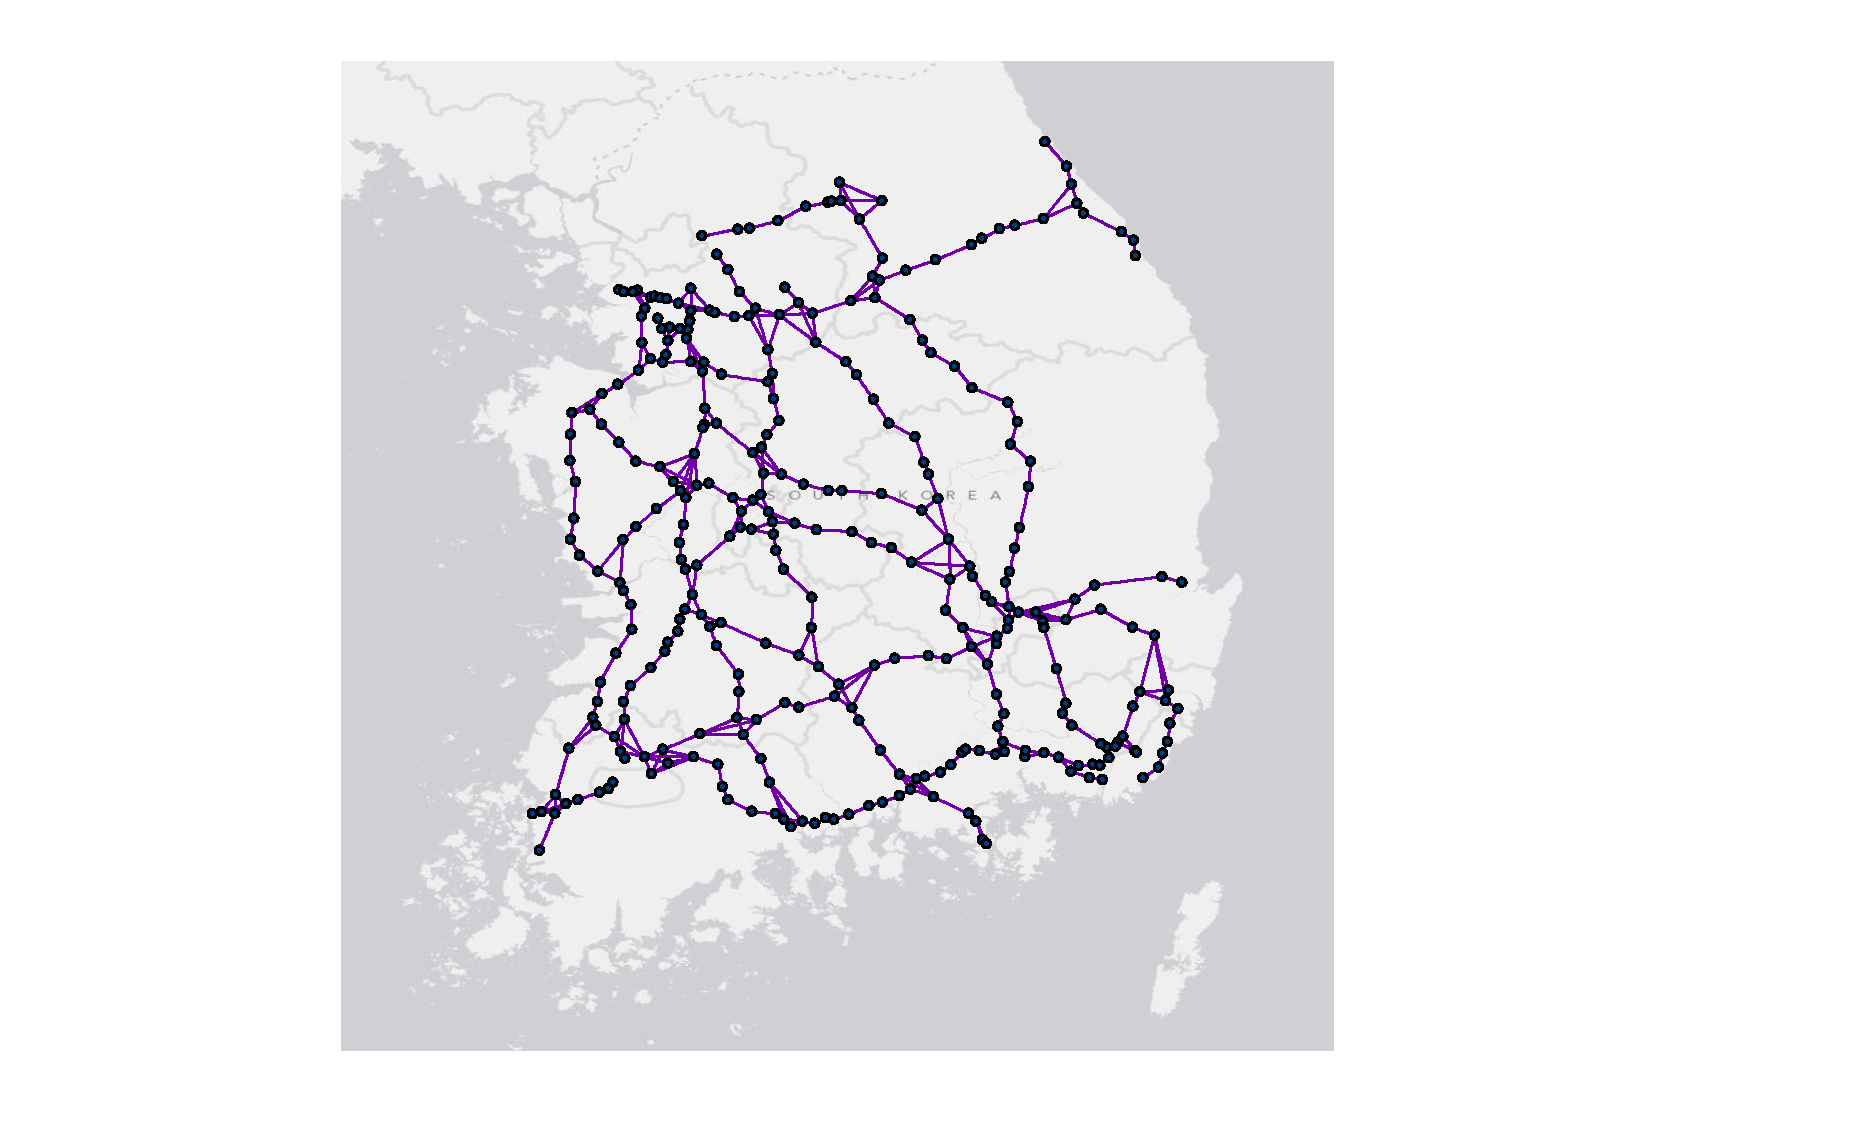
\includegraphics[width=\textwidth]{map}
\caption{Vector-based PDF}
\label{fig:map-pdf}
\end{subfigure}
%
\begin{subfigure}[b]{0.4\textwidth}
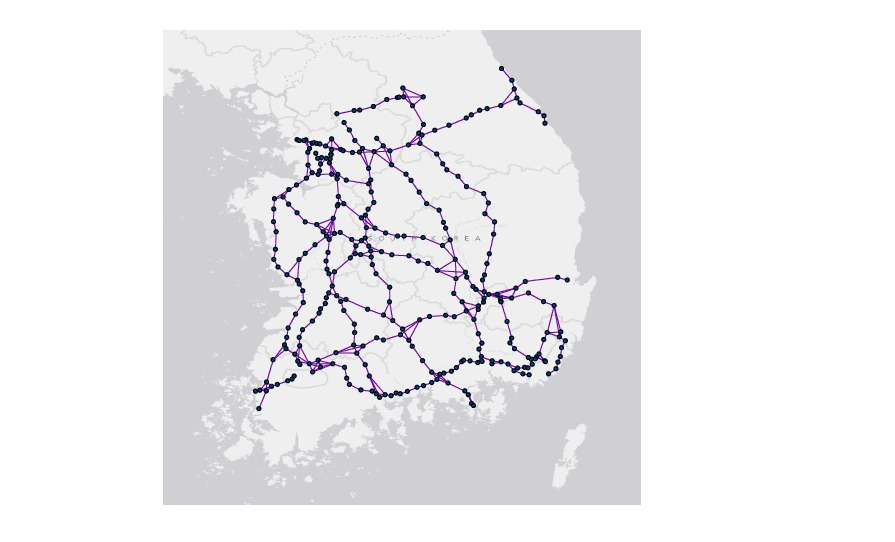
\includegraphics[width=\textwidth]{map-jpg}
\caption{PDF converted from JPG}
\label{fig:map-jpg}
\end{subfigure}
\caption{Figures side by side using \texttt{subfigure}. Zoom in and out to see the difference.}
\label{fig:side-by-side}
\end{figure}



\section{Concluding Remarks}

Some guidelines are provided in \url{http://stom.chkwon.net/latex}. If you have questions regarding \LaTeX, go to \url{http://tex.stackexchange.com} and ask questions to experts. I go there every day. This document has appendices. Appendix \ref{appendix:drawing} has some interesting materials.




\section*{Acknowledgement}
Thank you for reading this. This document was not supported by any agency.


\paragraph{Acknowledgement} 
Thank you for reading this. This document was not supported by any agency.




% Bibliography
\bibliographystyle{ormsv080-ck}		% Bibliography style. Journals/conferences may require something different
\bibliography{sample_ref}			% Your .bib filename goes here


% If you need appendices.
\newpage
\renewcommand{\appendixpagename}{Appendix}

\appendix
\appendixpage

This is appendix.

\section{Proofs} \label{appendix:proofs}

You may want to collect proofs for theorems here. This is Appendix \ref{appendix:proofs}.

\section{Data} \label{appendix:data}

Or maybe some data. This is Appendix \ref{appendix:data}.

\section{Drawing} \label{appendix:drawing}

You can also draw some figures within LaTeX. You can put it between text like this:
\begin{center}
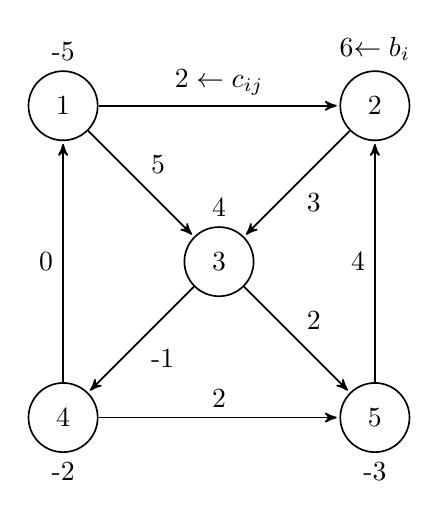
\begin{tikzpicture}[->,>=stealth',shorten >=1pt,auto,node distance=2.8cm,
                    semithick]

  \node[state] (node3) [label=above:4] {3};
  \node[state] (node1) [above left of=node3, label=above:-5] {1};
  \node[state] (node2) [above right of=node3, label=above:6$\leftarrow b_i$] {2};  
  \node[state] (node4) [below left of=node3, label=below:-2] {4};
  \node[state] (node5) [below right of=node3, label=below:-3] {5};

  \path (node1) edge node {$2\leftarrow c_{ij}$} (node2)
        (node1) edge node {5} (node3)
        (node2) edge node {3} (node3)
        (node3) edge node {2} (node5)
        (node3) edge node {-1} (node4)
        (node4) edge node {0} (node1)
        (node4) edge node {2} (node5)
        (node5) edge node {4} (node2)
        ;
\end{tikzpicture}
\end{center}
You can also put them in figures like Figures \ref{fig:network2} and \ref{fig:network3}. You can also draw a network that is slightly more graphical as in Figure \ref{fig:some_network}. You can even draw a digram that is as complicated as Figure \ref{fig:complicated}.








\begin{figure}
\begin{center}
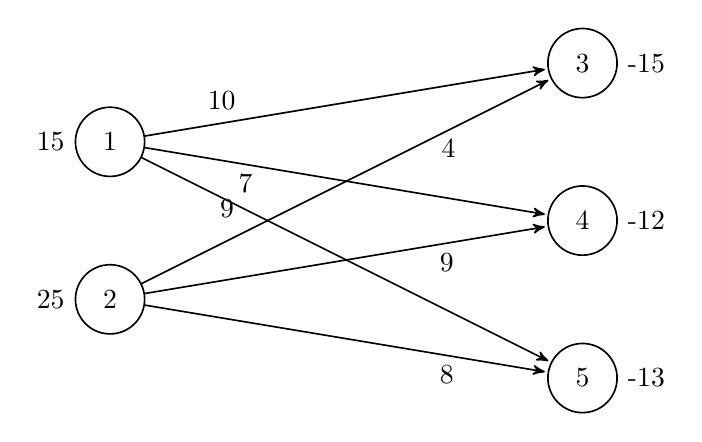
\begin{tikzpicture}[->,>=stealth',shorten >=1pt,auto,node distance=2.8cm,
                    semithick]

  \node[state] at(1,5) (node1) [label=left:15] {1};
  \node[state] at(1,3) (node2) [label=left:25] {2};
  \node[state] at(7,6) (node3) [label=right:-15] {3};
  \node[state] at(7,4) (node4) [label=right:-12] {4};  
  \node[state] at(7,2) (node5) [label=right:-13] {5};    

  \path (node1) edge node [near start]{10} (node3)
        (node1) edge node [near start, below]{7} (node4)
        (node1) edge node [near start, left]{9} (node5)
        (node2) edge node [near end, below]{4} (node3)
        (node2) edge node [near end, below]{9} (node4)
        (node2) edge node [near end, below]{8} (node5)
        ;

\end{tikzpicture}
\end{center}
\caption{Some network 2}
\label{fig:network2}
\end{figure}


\begin{figure}
\begin{center}
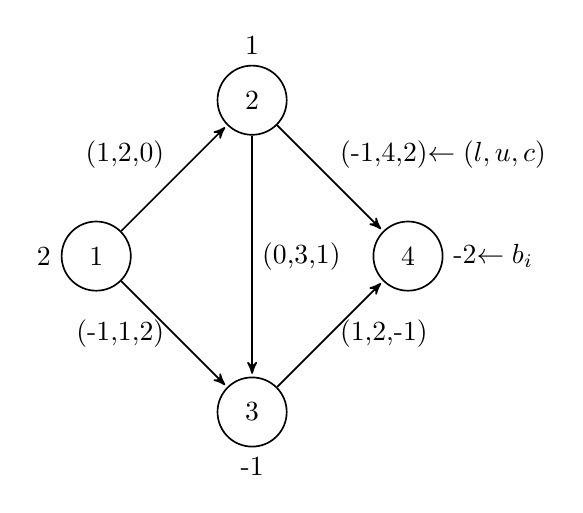
\begin{tikzpicture}[->,>=stealth',shorten >=1pt,auto,node distance=2.8cm,
                    semithick]

  \node[state] (node1) [label=left:2] {1};
  \node[state] (node2) [above right of=node1, label=above:1] {2};
  \node[state] (node3) [below right of=node1, label=below:-1] {3};
  \node[state] (node4) [below right of=node2, label=right:-2$\leftarrow b_i$] {4};

  \path (node1) edge node {(1,2,0)} (node2)
  		(node1) edge node [left] {(-1,1,2)} (node3)
  		(node2) edge node {(0,3,1)} (node3)
  		(node2) edge node {(-1,4,2)$\leftarrow(l,u,c)$} (node4)
  		(node3) edge node [right] {(1,2,-1)} (node4)
        ;
\end{tikzpicture}
\end{center}
\caption{Some network 3}
\label{fig:network3}
\end{figure}












\begin{figure} \centering
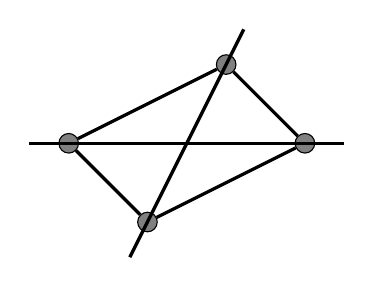
\begin{tikzpicture}[scale=1]
\tikzset{
    extended line/.style={
        to path={
            ($(\tikztostart)!-#1!(\tikztotarget)$) --  ($(\tikztotarget)!-#1!(\tikztostart)$) \tikztonodes
        }
    }
}
\tikzstyle{every node}=[circle, draw, fill=black!50,
                        inner sep=2.5pt, minimum width=4pt]
                        
\node (n1) at (2,3) {};
\node (n2) at (3,5) {};
\node (n3) at (1,4) {};
\node (n4) at (4,4) {};

\draw [very thick] (n1) to[extended line=0.5cm] (n2);
\draw [very thick] (n3) to[extended line=0.5cm] (n4);
\draw [very thick] (n1) -- (n3);
\draw [very thick] (n2) -- (n4);
\draw [very thick] (n1) -- (n4);
\draw [very thick] (n2) -- (n3);
\end{tikzpicture}
\caption{Some network}
\label{fig:some_network}
\end{figure}














\begin{figure}\centering
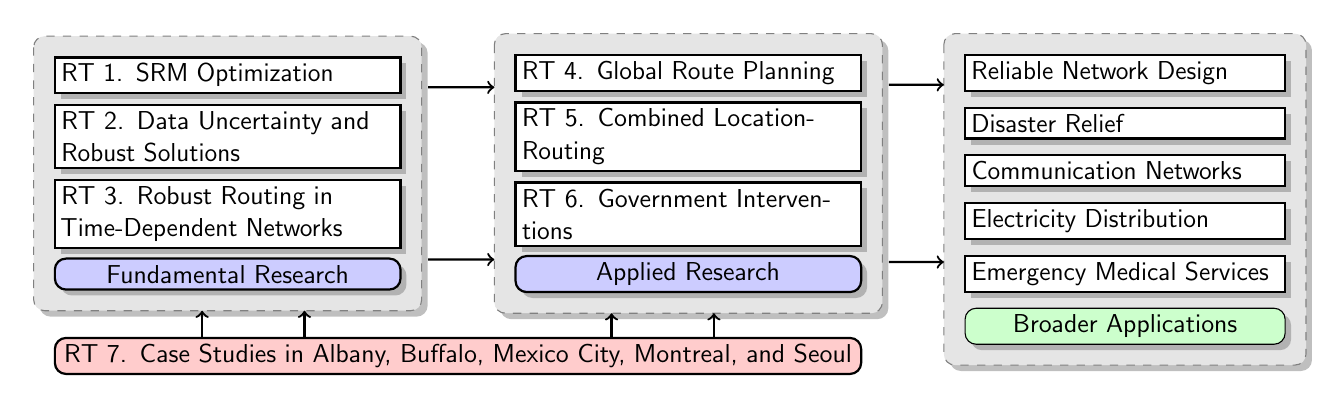
\begin{tikzpicture}[scale=0.65, transform shape, font=\Large\sffamily]

\tikzstyle{masterbox} = [inner sep=0]
\tikzstyle{bigbox} = [drop shadow, black, fill=gray!20!white,draw,inner sep=3.6pt, inner sep=7.5pt]
\tikzstyle{taskbox} = [drop shadow, thick, black, fill=white,draw, text width=6.5cm, inner sep=3.6pt]
\tikzstyle{researchbox} = [drop shadow, thick, black, fill=blue!20!white,draw,rounded corners, text width=6.5cm, text centered, inner sep=3.6pt]
\tikzstyle{babox} = [drop shadow, thick, black, fill=white,draw, text width=6cm, inner sep=3.6pt]
\tikzstyle{broaderbox} = [drop shadow, black, fill=green!20!white,draw,rounded corners, text width=6cm, text centered, inner sep=3.6pt]
\tikzstyle{casebox} = [thick, black, fill=red!20!white,draw,rounded corners, text width=15.5cm, text centered,inner sep=3.6pt]

\node[casebox] (case) {
	RT 7. Case Studies in Albany, Buffalo, Mexico City, Montreal, and Seoul
};

\node[researchbox, above=1.6cm of case.west, anchor=west] (fr) {Fundamental Research};
\node[taskbox, above=3.2cm of fr] (rt1) {RT 1. SRM Optimization};
\node[taskbox, below=0.2cm of rt1] (rt2) {RT 2. Data Uncertainty and Robust Solutions};
\node[taskbox, below=0.2cm of rt2] (rt3) {RT 3. Robust Routing in Time-Dependent Networks};

\begin{pgfonlayer}{background}
	\path (rt1.west |- rt1.north)+(-0.4,0.4) node (box1a) {};
	\path (fr.east |- fr.south)+(0.4,-0.4) node (box1b) {};
	\path [fill=black!10, drop shadow, rounded corners, draw=black!50, dashed] (box1a) rectangle (box1b); 
\end{pgfonlayer}	
	
\node[researchbox, above=1.6cm of case.east, anchor=east] (er) {Applied Research};
\node[taskbox, above=3.2cm of er] (rt4) {RT 4. Global Route Planning};
\node[taskbox, below=0.2cm of rt4] (rt5) {RT 5. Combined Location-Routing};
\node[taskbox, below=0.2cm of rt5] (rt6) {RT 6. Government Interventions};
	
\begin{pgfonlayer}{background}
	\path (rt4.west |- rt4.north)+(-0.4,0.4) node (box2a) {};
	\path (er.east |- er.south)+(0.4,-0.4) node (box2b) {};
	\path [fill=black!10, drop shadow, rounded corners, draw=black!50, dashed] (box2a) rectangle (box2b); 
\end{pgfonlayer}	

\path (box1a -| box1b) + (0,-1cm) node (box1c) {};
\path (box1b) + (0,1cm) node (box1d) {};
\draw[->,thick] (box1c) -- (box1c -| box2a);
\draw[->,thick] (box1d) -- (box1d -| box2a) ;


\node[babox, right=2cm of rt4] (ba1) {Reliable Network Design};
\node[babox, below=0.3cm of ba1] (ba2) {Disaster Relief};
\node[babox, below=0.3cm of ba2] (ba3) {Communication Networks};
\node[babox, below=0.3cm of ba3] (ba4) {Electricity Distribution};	
\node[babox, below=0.3cm of ba4] (ba5) {Emergency Medical Services};	
\node[broaderbox, below=0.3cm of ba5] (ba) {Broader Applications};	
	
\begin{pgfonlayer}{background}
	\path (ba1.west |- ba1.north)+(-0.4,0.4) node (box3a) {};
	\path (ba.east |- ba.south)+(0.4,-0.4) node (box3b) {};
	\path [fill=black!10, drop shadow, rounded corners, draw=black!50, dashed] (box3a) rectangle (box3b); 
\end{pgfonlayer}

\path (box2a -| box2b) + (0,-1cm) node (box2c) {};
\path (box2b) + (0,1cm) node (box2d) {};
\draw[->,thick] (box2c) -- (box2c -| box3a);
\draw[->,thick] (box2d) -- (box2d -| box3a) ;


		
\draw[->,thick] ([xshift=-5cm]case.north) -- ([xshift=-5cm]case.north |- box1b);
\draw[->,thick] ([xshift=-3cm]case.north) -- ([xshift=-3cm]case.north |- box1b);		

\draw[->,thick] ([xshift=5cm]case.north) -- ([xshift=5cm]case.north |- box2b);
\draw[->,thick] ([xshift=3cm]case.north) -- ([xshift=3cm]case.north |- box2b);	
		
\end{tikzpicture}
\caption{Complicated diagram}
\label{fig:complicated}
\end{figure}



\end{document}







%

